\documentclass{ximera}

\graphicspath{{./}{thePythagoreanTheorem/}{deMoivreSavesTheDay/}{complexNumbersFromDifferentAngles/}}

\usepackage{tikz}
\usepackage{tkz-euclide}
\usetkzobj{all}
\tikzstyle geometryDiagrams=[ultra thick,color=blue!50!black]
\newcommand{\tri}{\triangle}
\renewcommand{\l}{\ell}
\renewcommand{\P}{\mathcal{P}}
\newcommand{\R}{\mathbb{R}}
\newcommand{\Q}{\mathbb{Q}}

\newcommand{\Z}{\mathbb Z}

\renewcommand{\vec}{\mathbf}
\renewcommand{\d}{\,d}



%% Egyptian symbols

\usepackage{multido}
\newcommand{\egmil}[1]{\multido{\i=1+1}{#1}{
\includegraphics[scale=.1]{egyptian/egypt_person.pdf}\hspace{0.5mm}}}
\newcommand{\eghuntho}[1]{\multido{\i=1+1}{#1}{
\includegraphics[scale=.1]{egyptian/egypt_fish.pdf}\hspace{0.5mm}}}
\newcommand{\egtentho}[1]{\multido{\i=1+1}{#1}{
\includegraphics[scale=.1]{egyptian/egypt_finger.pdf}\hspace{0.5mm}}}
\newcommand{\egtho}[1]{\multido{\i=1+1}{#1}{
\includegraphics[scale=.1]{egyptian/egypt_lotus.pdf}\hspace{0.5mm}}}
\newcommand{\eghun}[1]{\multido{\i=1+1}{#1}{
\includegraphics[scale=.1]{egyptian/egypt_scroll.pdf}\hspace{0.5mm}}}
\newcommand{\egten}[1]{\multido{\i=1+1}{#1}{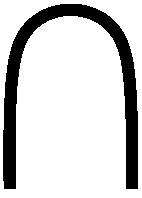
\includegraphics[scale=.1]{egyptian/egypt_heel.pdf}\hspace{0.5mm}}}
\newcommand{\egone}[1]{\multido{\i=1+1}{#1}{
\includegraphics[scale=.1]{egyptian/egypt_stroke.pdf}\hspace{0.5mm}}}
\newcommand{\egyptify}[7]{
 \multido{\i=1+1}{#1}{
\includegraphics[scale=.1]{egyptian/egypt_person.pdf}\hspace{0.5mm}}
 \multido{\i=1+1}{#2}{
\includegraphics[scale=.1]{egyptian/egypt_fish.pdf}\hspace{0.5mm}}
 \multido{\i=1+1}{#3}{
\includegraphics[scale=.1]{egyptian/egypt_finger.pdf}\hspace{0.5mm}}
 \multido{\i=1+1}{#4}{
\includegraphics[scale=.1]{egyptian/egypt_lotus.pdf}\hspace{0.5mm}}
 \multido{\i=1+1}{#5}{
\includegraphics[scale=.1]{egyptian/egypt_scroll.pdf}\hspace{0.5mm}}
 \multido{\i=1+1}{#6}{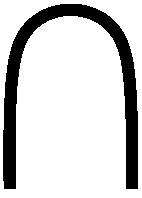
\includegraphics[scale=.1]{egyptian/egypt_heel.pdf}\hspace{0.5mm}}
 \multido{\i=1+1}{#7}{
\includegraphics[scale=.1]{egyptian/egypt_stroke.pdf}\hspace{0.5mm}}
 \hspace{.5mm}
}




\title{Bernoulli, Euler, and series}

\begin{document}
\begin{abstract}
Here we see some topics that both Bernoulli and Euler were interested in.
\end{abstract}
\maketitle

While Leibniz was investigating the sum of the reciprocals of the
triangular numbers, Johann Bernoulli was investigating the sum of the
reciprocals of the integers:
\[
1 + \frac{1}{2} + \frac{1}{3} + \frac{1}{4} + \frac{1}{5} + \frac{1}{6} + \frac{1}{7}+\cdots
\]
This is called the \textit{harmonic series}.  Johann Bernoulli's proof
started with the following definitions:

\begin{align*}
A &= \frac{1}{2} + \frac{1}{3} + \frac{1}{4} + \frac{1}{5} + \frac{1}{6} + \frac{1}{7} + \cdots\\
B &= \frac{1}{2} + \frac{2}{6} + \frac{3}{12} + \frac{4}{20} + \frac{5}{30} + \frac{6}{42} + \cdots
\end{align*}

\begin{question}
Next he defined
\[
{\renewcommand{\arraystretch}{2.5}
\arraycolsep=1.4pt
\begin{array}{ccccccccccccccc}
C & = & \frac{1}{2} & + & \frac{1}{6} & + & \frac{1}{12} & + & \frac{1}{20} & + & \frac{1}{30} & + & \frac{1}{42} & + & \cdots\\
D & = &             &   & \frac{1}{6} & + & \frac{1}{12} & + & \frac{1}{20} & + & \frac{1}{30} & + & \frac{1}{42} & + & \cdots\\
E & = &             &   &             &   & \frac{1}{12} & + & \frac{1}{20} & + & \frac{1}{30} & + & \frac{1}{42} & + & \cdots\\
F & = &             &   &             &   &              &   & \frac{1}{20} & + & \frac{1}{30} & + & \frac{1}{42} & + & \cdots
\end{array}}
\]
Compute $C$, $D$, $E$, and $F$. Can you convince yourself that the pattern will continue?
\end{question}

\begin{question}
Explain why
\[
C + D + E + F + \cdots = A.
\]
\end{question}

\begin{question}
Explain why
\[
C + D + E + F + \cdots = A+1.
\]
\end{question}

\begin{question}
Explain why Johann concluded that the series
\[
1 + \frac{1}{2} + \frac{1}{3} + \frac{1}{4} + \frac{1}{5} + \frac{1}{6} + \frac{1}{7}+\cdots
\]
diverges. 
\end{question}


\begin{question}
Explicitly explain how would a calculus student could see that the
series
\[
1 + \frac{1}{2} + \frac{1}{3} + \frac{1}{4} + \frac{1}{5} + \frac{1}{6} + \frac{1}{7}+\cdots
\]
diverges.
\end{question}

\begin{question}
Do you know any other proofs that the harmonic series diverges?
\end{question}


On the other hand Euler investigated this sum:
\[
1 + \frac{1}{4} + \frac{1}{9} + \frac{1}{16} + \frac{1}{25} + \frac{1}{36} + \frac{1}{49}\cdots
\]
or the sum of the reciprocals of the square numbers. 


\begin{question}
Consider:
\[
f(x) = 1 - \frac{x^2}{3!} + \frac{x^4}{5!}-\frac{x^6}{7!} + \frac{x^8}{9!} - \frac{x^{10}}{11!} + \dots
\]
Can you explain why 
\[
f(x) = \frac{\sin(x)}{x}\qquad x \ne 0?
\]
\end{question}


\begin{question}
Let $g(x)$ be a polynomial with roots $a_1,\dots, a_n$. What are the factors of $g(x)$?
\end{question}

\begin{question}
What exactly are the roots of $f(x)$?
\end{question}

\begin{question}
Explain why:
\[
f(x) = \bigg(1-\frac{x}{\pi} \bigg)\bigg(1-\frac{x}{-\pi} \bigg)\bigg(1-\frac{x}{2\pi} \bigg)\bigg(1-\frac{x}{-2\pi} \bigg)\bigg(1-\frac{x}{3\pi} \bigg)\bigg(1-\frac{x}{-3\pi} \bigg) \cdots
\]
\end{question}

\begin{question}
Explain why:
\[
f(x) = \prod_{n=1}^\infty \left(1 - \frac{x^2}{n^2\pi^2} \right)
\]
\end{question}

\begin{question}
Explain why:
\[
f(x) = 1 - x^2 \sum_{n=1}^\infty \frac{1}{n^2\pi^2} 
+ x^4 \bigg(\cdots\bigg)  - x^6 \bigg(\cdots\bigg)  + \cdots
\]
\end{question}


\begin{question}
Explain why:
\[
\sum_{n=1}^\infty \frac{1}{n^2}= \frac{\pi^2}{6}.
\]
\end{question}

\begin{exploration}[Bonus!]
Compute
\[
\sum_{n=1}^\infty \frac{1}{n^3}.
\]
\end{exploration}

\end{document}
